{\color{blue} 
%Dans ce chapitre, nous nous intéressons aux fluctuations de la distribution de rapidité \( \delta \rho \) autour d'une distribution de référence \( \rho^c \), qui maximise la contribution à la fonction de partition des états, exprimée comme une fonctionnelle de la distribution \( \rho \) : 

%La fonction de partition des états, s'exprime comme une fonctionnelle de la distribution \( \rho \) : 

%\begin{eqnarray*}\Xi & = & \sum_\rho \exp \left( -\mathcal{A}(\rho) \right).\end{eqnarray*}  

%Dans la section {\em \bf Entropie de Yang-Yang} (\ref{??}), l'action \( \mathcal{A}(\rho) \) s'écrit sous la forme :  

%\begin{eqnarray*}\mathcal{A}(\rho) & \doteq & - L\mathcal{S}_{YY}(\rho) + L\int f(\theta) \rho (\theta) \, d\theta,		\end{eqnarray*}  

%où \( \mathcal{S}_{YY} \) est la fonctionnelle d'entropie de Yang-Yang, définie dans (\ref{??}), et \( f \) est la fonction paramétrant les charges, introduite dans (\ref{??}).  
}

La fonction de partition des états s’exprime comme une fonctionnelle de la distribution de rapidité \( \rho \) :
\begin{eqnarray*}
	\Xi & = & \sum_\rho \exp\left( -\mathcal{A}(\rho) \right).
\end{eqnarray*}

Dans la section \textit{\textbf{Entropie de Yang-Yang}} (\ref{??}), nous avons montré que l’action \( \mathcal{A}(\rho) \) s’écrit sous la forme :
\begin{eqnarray*}
	\mathcal{A}(\rho) & \doteq & - L\mathcal{S}_{YY}(\rho) + L \int f(\theta)\, \rho(\theta) \, d\theta,
\end{eqnarray*}
où \( \mathcal{S}_{YY} \) désigne la fonctionnelle d'entropie de Yang-Yang, définie en (\ref{??}), et \( f \) la fonction génératrice associée aux charges conservées, introduite en (\ref{??}).

{\color{blue} 
%Dans cette même section {\em \bf Entropie de Yang-Yang} (\ref{??}), nous avons établi un lien entre \( f \) et distribution de référence \( \rho^c \), qui maximise la contribution à la fonction de partition des états .\\

}

Dans cette même section, nous avons également mis en évidence que la distribution \( \rho^c \) qui maximise la contribution à la fonction de partition correspond à un point stationnaire de l'action, et est entièrement déterminée par la fonction \( f \). Cette distribution \( \rho^c \) définit ainsi l’état macroscopique typique du système au sein de l’ensemble statistique considéré.

{\color{blue} 

%L'hypothèse qui après relaxation le système est décrit pas un GGE, est fondamantale dans notre compréhention, et a énormément d'implication. Et donc il est ittéressent de tester cette hyphotèse experimentalement.La distribution de rapidité moyenne $\rho^c$ ne permet pas de verifier que le GGE est bien l'enssemeble statistique adequa. En effet plein d'autre enssemble statistique donne la meme distribution de rapidité moyenne. Il faut donc aller au dela. Il faut regarder les fluctuation de distribution de rapidité \( \delta \rho \) autour \( \rho^c \)

%L'hypothèse selon laquelle, après relaxation, le système est décrit par un ensemble généralisé de Gibbs (GGE) constitue un pilier fondamental de notre compréhension des dynamiques hors équilibre dans les systèmes intégrables. Cette hypothèse a des implications théoriques majeures, et il est donc essentiel de la confronter à l'expérience. Cependant, la seule connaissance de la distribution de rapidité moyenne $\rho^c$ ne permet pas de valider cette description. En effet, plusieurs ensembles statistiques peuvent conduire à une même distribution moyenne. Pour distinguer le GGE des autres candidats, il est nécessaire d’aller au-delà et d’analyser les fluctuations de la distribution de rapidité, notées \( \delta \rho \), autour de la valeur moyenne \( \rho^c \).


%On veux tester si nos experience est décrit pas un GGE. Pour cela nous nous intéressons aux fluctuations de la distribution de rapidité \( \delta \rho \) autour \( \rho^c \).

%Nous poursuivons à présent avec cette définition de l'action de classe $\mathcal{C}^2$ et admetant une distribution critique $\rho^c$ tel que sa différentielle en ce point critique soit nulle $d\mathcal{A}_{\rho^c} = 0 $ (\ref{??}) de sorte que d'aprés la formule de Taylor-Youg %afin de déterminer les fluctuations autour de \( \Pi^c \). Pour cela, nous réécrivons l'action sous la forme :  

%Nous poursuivons en développant l'action autour de la  distribution  $\rho^c$. La différentielle de l'action en ce point  est nulle ($d\mathcal{A}_{\rho^c} = 0 $ (\ref{??})).D'aprés la formule de Taylor-Youg , à l'ordre 2 en $\delta \rho$,  l'action s'écrit avec une forme quadratique : % tel que sa différentielle en ce point critique soit nulle ,  de sorte que d'aprés la formulle de Taylor-Youg %afin de déterminer les fluctuations autour de \( \Pi^c \). Pour cela, nous réécrivons l'action sous la forme :  

%\begin{eqnarray*}  \mathcal{A}(\rho^c + \delta \rho) & \underset{ \delta \rho \to 0 }{=} & \mathcal{A}(\rho^c)  + \frac{1}{2} \left. \frac{\delta^2 \mathcal{A}}{\delta \rho^2} \right|_{\rho^c} (\delta \rho) + \mathcal{O}((\delta \rho)^3),  \end{eqnarray*}  

%une expression quadratique pour l'action à l'ordre dominant en \( \delta \Pi \) avec $\left. \frac{\delta^2 \mathcal{A}}{\delta \rho^2} \right|_{\rho^c}$ la forme quadratique définie positive (Fig (\ref{fig.fluctu.A})).

}





L’hypothèse selon laquelle, après relaxation, le système est décrit par un ensemble généralisé de Gibbs (GGE) constitue un fondement majeur de notre compréhension des dynamiques hors équilibre dans les systèmes intégrables. Cette hypothèse a des implications théoriques profondes et mérite d’être testée expérimentalement. Toutefois, la seule connaissance de la distribution de rapidité moyenne \( \rho^c \) ne permet pas de confirmer l'adéquation du GGE. En effet, plusieurs ensembles statistiques peuvent mener à une même valeur moyenne de \( \rho \). Pour lever cette ambiguïté, il est nécessaire d’étudier les fluctuations autour de la distribution typique, notées \( \delta \rho \), définies par \( \rho = \rho^c + \delta \rho \).

Afin de caractériser ces fluctuations, nous développons l’action \( \mathcal{A}(\rho) \) au voisinage de \( \rho^c \). Par construction, \( \rho^c \) étant un point stationnaire, la différentielle première de \( \mathcal{A} \) en ce point est nulle : \( d\mathcal{A}_{\rho^c} = 0 \) (cf. équation~(\ref{??})). En appliquant le développement de Taylor-Young à l’ordre deux en \( \delta \rho \), nous obtenons :
\begin{eqnarray*}
	\mathcal{A}(\rho^c + \delta \rho) & \underset{ \delta \rho \to 0 }{=} & \mathcal{A}(\rho^c)  + \frac{1}{2} \left. \frac{\delta^2 \mathcal{A}}{\delta \rho^2} \right|_{\rho^c} (\delta \rho) + \mathcal{O}((\delta \rho)^3),
\end{eqnarray*}
où \( \left. \frac{\delta^2 \mathcal{A}}{\delta \rho^2} \right|_{\rho^c} \) désigne la forme linéaire symétrique (a priori définie positive) associée à la hessienne de l’action, illustrée en Fig.~(\ref{fig.fluctu.A}). Cette approximation quadratique constitue la base du traitement gaussien des fluctuations autour de l’état typique, permettant d’accéder aux corrélations et à la structure fine de l’ensemble statistique effectif.





\begin{figure}[H]
	\centering 
	\begin{tikzpicture}
		\begin{scope}[shift={(0,0)}]
			\begin{scope}[transform canvas={scale=0.6}]
				% Définition des couleurs avec les codes HTML
\definecolor{colorOne}{HTML}{443E46}
\definecolor{colorTwo}{HTML}{F6DEB8}
\definecolor{colorThree}{HTML}{908CA4}
\definecolor{colorFour}{HTML}{57659E}
\definecolor{colorFive}{HTML}{C57284}
\definecolor{colorSix}{HTML}{FF5B69}

% Raccourcis pour les couleurs
\def\colorOne{colorOne}
\def\colorTwo{colorTwo}
\def\colorThree{colorThree}
\def\colorFour{colorFour}
\def\colorFive{colorFive}
\def\colorSix{colorSix}

\def\colorslide{blue!50!black}



\begin{scope}
	% Tracer une courbe lisse entre des points
	\draw[shift={(0,0)} ,\colorOne]
		(-1 , 0 ) edge [thick,line width=0.8ex , ->,>=triangle 45  , \colorOne] node [pos = 1 , below ]{\huge$\rho$}( 5  , 0 )
	;
	\draw[shift={(0,0)}, color=\colorOne]
		(0, -1.0 ) edge [thick,line width=0.8ex , ->,>=triangle 45  ]node [pos=0.9,left=0.2cm ]{\huge$\mathcal{A}(\rho)$}( 0  , 5 )
	;
	\draw[]
		(2.5, 0.12 ) edge [thick,line width=0.8ex ,\colorThree ]node [pos=1,below  ]{\huge$\rho^c$} (2.5, -0.12 )	
	;
	
	\draw[]
		(2.5, -0.12 ) edge [thick,line width=0.4ex , dashed, \colorThree ] (2.5, 5.5 )
		(1.5, 1 ) edge [thick,line width=0.4ex , <->,>=triangle 45  , \colorThree ] (3.5, 1 )
		(-0.3,1) edge [thick,line width=0.4ex  , \colorThree ] node [pos=0,left ]{\huge$\mathcal{A}(\rho^c)$} (0.3, 1 )	
	;
    \draw[thick, line width=0.8ex , \colorFour] plot[smooth, tension=0.7] coordinates {
        (1, 5) (1.6 , 3 ) (2.5, 1) (3.5 , 3 )  (4, 5)
    };		
	
\end{scope}

	
			
			\end{scope}
			
			\draw[color = red , scale = 0.5 , draw = none  ] (-2 , -1) rectangle (5, 6) ; 	
		\end{scope}
		
		\begin{scope}[shift={(19,-1)}]
			\begin{scope}[transform canvas={scale=0.6}]
				% Définition des couleurs avec les codes HTML
\definecolor{colorOne}{HTML}{443E46}
\definecolor{colorTwo}{HTML}{F6DEB8}
\definecolor{colorThree}{HTML}{908CA4}
\definecolor{colorFour}{HTML}{57659E}
\definecolor{colorFive}{HTML}{C57284}
\definecolor{colorSix}{HTML}{FF5B69}

% Raccourcis pour les couleurs
\def\colorOne{colorOne}
\def\colorTwo{colorTwo}
\def\colorThree{colorThree}
\def\colorFour{colorFour}
\def\colorFive{colorFive}
\def\colorSix{colorSix}

\def\colorslide{blue!50!black}

\def\Occupation{
	\def\traitx{0.3}
	\def\traity{0.5}
	\draw[shift={(0,0)}]
		(-13.5 , 0 ) edge [thick,line width=0.8ex ]( -3.2  , 0 )
		( -3.2 - \traitx  , 0 - \traity ) edge [thick,line width=0.8ex ]( -3.2 + \traitx  , 0 + \traity  )
		( -2.8 - \traitx  , 0 - \traity ) edge [thick,line width=0.8ex ]( -2.8 + \traitx  , 0 + \traity  )
		(-2.8 , 0 ) edge [thick,line width=0.8ex ](2.8  , 0 )
		( 2.8 - \traitx  , 0 - \traity ) edge [thick,line width=0.8ex ]( 2.8 + \traitx  , 0 + \traity  )
		( 3.2 - \traitx  , 0 - \traity ) edge [thick,line width=0.8ex ]( 3.2 + \traitx  , 0 + \traity  )
		(3.2, 0 ) edge [thick,line width=0.8ex,->,>=triangle 45 , color = black ]node [pos=1.01,below  ]{\huge$\theta$}	( 13  , 0 )
	;
	\draw[shift={(0,0)}, color=\colorOne]
		(-10.5 , -1.5 ) edge [thick,line width=0.8ex , ->,>=triangle 45  ]( -10.5  , 4.5 )
	;
		
	\foreach \r in {1 , ... , 3 } {
%		\draw[
%		decoration={
%		markings,
%    	mark connection node=my node,
%    	mark=at position 0 with{\node [blue,transform shape] (my node) {\large \r};}},
%		color=gray, thick, 
%		line width=0.5ex] decorate { 
%            (-11.0, \r) -- (-10.1, \r )}
%        ;
        \draw[
			color=\colorOne,
			] 
            (-11.0, \r) edge[color=\colorThree , thick,line width=0.5ex] node [pos=-0.5 ]{\large\color{\colorFour} $\frac{\r}{\delta \theta}$ } (-10.3, \r )
        	;
	
	}
	

	
	% Graduation abcsisse 
	% Définitions des listes
% Definitions of the lists
\def\listetuple{-9/\theta_{1}, -8/\theta_{2} , -5/\theta_{3} , -2/\theta_{a-1} , 0/\theta_{a} , 1/\theta_{a+1} , 2/\theta_{a+2} ,  5/\theta_{N-4} , 7/\theta_{N-3},8/\theta_{N-1},9/\theta_{N} }
\def\listetrais{-12 , -11, -10, -9 , -8 , -7 ,  -6 , -5, -4.5,-4, -2 , -1, 0 , 0.5, 1, 2, 4 , 5 ,  6 , 7 , 8 ,8.5, 9 ,  10 , 11, 12 }

% Loop over listetrais
\foreach \r in \listetrais {
    % Initialize found variable to zero
    % Initialize found variable to zero
    %\pgfmathsetmacro\found{0}
    \global\def\found{0}
    \xdef\nomtheta{}
    
    % Check if \r is in listetuple
    \foreach \x/\y in \listetuple { 
        \ifdim \r pt=\x pt % If \r matches any \x in listetuple
            \global\def\found{1} ;
            \xdef\nomtheta{\y} % Set \nomtheta to the corresponding \y
            %\pgfmathsetmacro\found{1} % Set found to 1            
            %\global\pgfmathsetmacro\found{1}
        \fi
    }
    
    %\node [circle, draw, red] (A) at (\r, 2) {\found , $\nomtheta$};
    
    % Draw the line and display \nomtheta if found
    \ifnum\found=1
        \draw[color=\colorOne, thick, line width=0.5ex] 
            (\r, -0.3) -- (\r, 0.3) node[red , pos=-0.5] {\large $\nomtheta$};
         \filldraw[line width=0.5ex, color=\colorSix, outer color=\colorSix, inner color=\colorSix] 
            (\r, 0) circle (4pt);
    \else 
        % Draw without \nomtheta and add a blue circle if not found
        \draw[color=\colorOne, thick, line width=0.5ex] 
            (\r, -0.3) -- (\r, 0.3);
        \filldraw[line width=0.5ex, color=\colorSix, outer color=\colorTwo, inner color=\colorTwo] 
            (\r, 0) circle (4pt); 
    \fi
}

\def\listetrais{-9.5/\theta_{i-1}/2/3, -6.5/\theta_{i}/1/4  ,   -1.5/\theta_{j}/2/4 , 1.5/\theta_{j+1}/-1/3 , 3.5/\theta_{\ell-1}/1/3 , 6.5/\theta_{\ell}/3/4 , 9.5/\theta(\theta_{\ell+1})/-1/3 };



\foreach \r/\nomx/\y/\ys in \listetrais {
	\draw[
		decoration={
		markings,
    	mark connection node=my node,
    	mark=at position .5 with{\node [blue,transform shape] (my node) {\large \color{\colorFour} $\nomx$};}},
		color=\colorThree , thick, 
		line width=0.5ex] decorate { 
            (\r, 0.12) -- (\r, -1.2)}
        ;
     
     \ifdim \y pt > -1 pt 
     	\draw[
			decoration={
			markings,
    		mark connection node=my node,
    		mark=at position .5 with{\node [blue,transform shape] (my node) {\large \color{\colorFour} $\Pi(\nomx) $};}},
			color=\colorThree, thick, 
			line width=0.5ex] decorate { 
            (\r, \y) -- (\r +3, \y)}
        ;
        \draw[
			decoration={
			markings,
    		mark connection node=my node,
    		mark=at position .5 with{\node [blue,transform shape] (my node) {\large \color{\colorFive} $\Pi_s(\nomx) $};}},
			color=\colorFive, thick, 
			line width=0.5ex] decorate { 
            (\r, \ys) -- (\r +3, \ys)}
        ;
     \fi 
     \ifdim \r pt= -1.5 pt
     	\draw[
     		decoration={
			markings,
    		mark connection node=my node,
    		mark=at position .5 with{\node [blue,transform shape] (my node) {\large \color{\colorFour}  $\delta \theta $};},
    		%mark=at position 0.1  with {\arrow[blue, line width=0.5ex]{<}},
    		%mark=at position 1  with {\arrow[blue, line width=0.5ex]{>}}
    		},
        	color=\colorThree,
        	thick,
        	line width=0.5ex,
        	%arrows={Computer Modern Rightarrow[line cap=round]-Computer Modern Rightarrow[line cap=round]}
   			](\r, -1.2) edge[arrows={Computer Modern Rightarrow[line cap=round]-}] (\r + 0.4, -1.2)decorate {
    		(\r, -1.2) -- (\r + 3, -1.2)}(\r + 2, -1.2) edge[arrows={-Computer Modern Rightarrow[line cap=round]}] (\r + 3, -1.2)
    		;
    \fi
			
	
}


			
}


\begin{scope}
	%\draw[help lines , width=1.5ex] (-8,-3) grid (8,3);\draw[help lines ,width=0.5ex , opacity = 0.5] (-3,-3) grid[step=0.1] (3,3));
	
	%\draw[help lines] 
	%	(-3,-3) edge[width=1.5ex] grid (3,3)	
	%	(-3,-3) edge[width=0.5ex , opacity = 0.5] grid (3,3)	
	%;
	\begin{scope}[shift={(0,1)},rotate=0,opacity=1,color=black]
		\Occupation	
		
		%\node[anchor=east, font=\bfseries] at (-11, 0) {\color{red}\large (T = 0 )} ;	
	\end{scope}
	
	
	
	
	\begin{scope}[shift={(-10.5,7)},rotate=0,opacity=1,color=black]
	
	\begin{scope}[shift={(-0,0)},rotate=0,opacity=1,color=black]
	
		\draw[shift={(0,0)} ,line width=1ex,rounded corners = 1ex,color=\colorOne , opacity =1 ,fill=\colorOne!00 , pattern={north east lines} , pattern color=\colorOne!00 ]
			(0 , -1 ) rectangle (5,1)
		;
		

		\begin{scope}[shift={(0.5,0.5)}]
			\draw[color=\colorOne, thick, line width=0.5ex] 
            (0, -0.3) -- (0, 0.3) ;
            \filldraw[line width=0.5ex, color=\colorSix, outer color=\colorSix, inner color=\colorSix] 
            (0, 0) circle (4pt);
            
            \node[anchor=west, font=\bfseries] at (0.2, 0) {\color{\colorSix}\large : quasi-particule};
		\end{scope}
		
		\begin{scope}[shift={(0.5,-0.5)}]
			\draw[color=\colorOne, thick, line width=0.5ex] 
            (0, -0.3) -- (0, 0.3) ;
            \filldraw[line width=0.5ex, color=\colorSix, outer color=\colorTwo, inner color=\colorTwo] 
            (0, 0) circle (4pt);
            
            \node[anchor=west, font=\bfseries] at (0.2, 0) {\color{\colorSix}\large : hole};
		\end{scope}

	\end{scope}
	
	\begin{scope}[shift={(6,0)},rotate=0,opacity=1,color=black]	
		
		\draw[shift={(0,0)} ,line width=1ex,rounded corners = 1ex,color=\colorOne , opacity =1 ,fill=\colorOne!00 , pattern={north east lines} , pattern color=\colorOne!00 ]
			(0 , -1 ) rectangle (7.5,1)
		;
		
		\node[anchor=west] at (0.5, 0.5) {\color{\colorFour}\large $\Pi$ };\node[anchor=west, font=\bfseries] at (1, 0.5) {\color{\colorFour}\large : quasi-particule distribution};
		
		\node[anchor=west] at (0.5, -0.5) {\color{\colorFour}\large $\Pi_h$ };\node[anchor=west, font=\bfseries] at (1, -0.5) {\color{\colorFour}\large  : hole distribution};
		
	\end{scope}
	
	\begin{scope}[shift={(14.5,0)},rotate=0,opacity=1,color=black]	
		
		\draw[shift={(0,0)} ,line width=1ex,rounded corners = 1ex,color=\colorOne , opacity =1 ,fill=\colorOne!00 , pattern={north east lines} , pattern color=\colorOne!00 ]
			(0 , -0.5 ) rectangle (7.0,0.5)
		;
		
		\node[anchor=west] at (0.2, 0) {\color{\colorFour}\large ${\color{\colorFive}\Pi_s} = \Pi + \Pi_h $ } node[anchor=west , font=\bfseries] at (3.1 , 0 )  {\color{\colorFour}\large {\color{\colorFive} : density of states}};
		
	\end{scope}
	
	
	\end{scope}


		
	
\end{scope}

	
			
			\end{scope}
			\begin{scope}[scale=1]
				\draw[color = red , scale = 1 , draw = none  ] (-1 , -1) rectangle (5, 5) ; 
			\end{scope}	
		\end{scope}

		
				
			
	\end{tikzpicture}	
	\captionsetup{skip=10pt} % Ajoute de l’espace après la légende
	\label{fig.fluctu.A}
\end{figure}

{\color{blue}
%On discrétise l'axe des rapidités en  petite cellule de rapidité $[\theta, \theta+\delta\theta]$, qui contient $L\rho(\theta) \delta \theta$ rapidités. 
	



%Avec ces petites tranches, la forme quadratique s’écrit :

%\begin{eqnarray*}
%    \left. \frac{\delta^2 \mathcal{A}}{{\delta \rho}^2} \right|_{\rho^c}(\delta \rho ) &=&  \sum_{a,b \mid \text{tranche}}  
%    \delta \rho(\theta_a)  \frac{\partial^2 \mathcal{A}}{\partial \delta \rho(\theta_a) \partial \delta \rho(\theta_b) } (\rho^c)  \delta \rho(\theta_b).
%\end{eqnarray*}
%Les fluctuations s’écrivent donc :

%\begin{eqnarray*}
%    \langle \delta \rho ( \theta) \delta \rho ( \theta') \rangle &=&  
%    \frac{ \int d\delta \rho \, \delta \rho(\theta) \delta \rho ( \theta') 
%    \exp \left( - \frac{1}{2} \sum_{a,b \mid \text{tranche}}  
%    \delta \rho(\theta_a) \frac{\partial^2 \mathcal{A}}{\partial \delta \rho(\theta_a) \partial \delta \rho(\theta_b) } (\rho^c)  \delta \rho(\theta_b) \right) }
%    { \int d\delta \Pi  
%    \exp \left( - \frac{1}{2} \sum_{a,b \mid \text{tranche}}  
%    \delta \rho(\theta_a) \frac{\partial^2 \mathcal{A}}{\partial \delta \rho(\theta_a) \partial \delta \rho(\theta_b) } (\rho^c)  \delta \rho(\theta_b) \right) } \\
%    &=& \left( \mathbf{A}^{-1} \right)_{\theta , \theta'}
%\end{eqnarray*}


%\begin{aff}

%\begin{eqnarray*}\langle \delta \rho ( \theta) \delta \rho ( \theta') \rangle &=& 	\left( \mathbf{A}^{-1} \right)_{\theta , \theta'}\end{eqnarray*}

	
%avec la  {\em matrice hessienne} $\mathbf{A}_{\theta , \theta'} \equiv \frac{\partial^2 \mathcal{A}}{\partial \delta \rho(\theta) \partial \delta \rho(\theta') }(\rho^c)$, au point critique/ qui maximise la probabilité  $\rho^c=\rho^c_s \nu^c $, s'écrit

%avec la  matrice $\mathbf{A}_{\theta , \theta'} \equiv \frac{\partial^2 \mathcal{A}}{\partial \delta \rho(\theta) \partial \delta \rho(\theta') }(\rho^c)$, qui maximise la probabilité  $\rho^c=\rho^c_s \nu^c $, s'écrit

%\begin{eqnarray*}
%	\operator{A} & = & \operator{A}^{(0)} + \delta \theta \operator{V}
%\end{eqnarray*}

%avec 

%\begin{eqnarray*}
%	A^{(0)}_{\theta , \theta'}  & = &  L\delta \theta \left ( \frac{ 1}{\rho^c_s ( 1  - \nu^c ) \nu^c } \right )(\theta)    \delta({\theta - \theta '})	,\\
%	V_{\theta , \theta'}  &= & L \delta \theta \left \{ - \left [ \left ( \frac{1}{\rho^c_s( 1 - \nu^c) } \right ) ( \theta)  +  \left ( \frac{1}{\rho^c_s( 1 - \nu^c) } \right ) ( \theta' )\right ] \frac{ \Delta( \theta'- \theta )}{ 2 \pi } + \int d\theta''  \left ( \frac{\nu^c}{\rho^c_s( 1 - \nu^c) } \right )(\theta'') \frac{\Delta(\theta''- \theta)}{2 \pi}\frac{\Delta(\theta''- \theta')}{2 \pi}   \right \} 	
%\end{eqnarray*}

%\end{aff}

}

\section{Fluctuations autour du profil stationnaire}

Dans les systèmes intégrables à grand nombre de particules, la description hydrodynamique est régie par la densité de rapidité \( \rho(\theta) \), qui encode la répartition des quasi-particules sur l’axe des rapidités \( \theta \). À l'équilibre, le profil stationnaire \( \rho^c(\theta) \) maximise la probabilité d’observer une configuration donnée. On s’intéresse ici aux fluctuations autour de ce profil stationnaire, et plus précisément aux corrélations à deux points des fluctuations \( \delta \rho(\theta) = \rho(\theta) - \rho^c(\theta) \).

Pour ce faire, on discrétise l’axe des rapidités en petites cellules \( [\theta, \theta + \delta\theta] \), chacune contenant un nombre moyen de quasi-particules donné par \( L \rho(\theta) \, \delta\theta \), où \( L \) désigne la taille du système. 

Dans cette discrétisation, le développement quadratique de l’action \( \mathcal{A}[\rho] \) autour du profil stationnaire \( \rho^c \) s’écrit comme un produis scalaire:

\begin{equation*}
    \left. \frac{\delta^2 \mathcal{A}}{{\delta \rho}^2} \right|_{\rho^c}(\delta \rho ) =  
    \sum_{a,b} \delta \rho(\theta_a)  
    \frac{\partial^2 \mathcal{A}}{\partial \delta \rho(\theta_a) \, \partial \delta \rho(\theta_b)} \Big|_{\rho^c} 
    \delta \rho(\theta_b).
\end{equation*}

Cette structure quadratique mène naturellement à une intégrale fonctionnelle gaussienne pour la probabilité des fluctuations. Les corrélations à deux points des fluctuations s’expriment alors comme :

\begin{equation*}
    \langle \delta \rho(\theta) \, \delta \rho(\theta') \rangle 
    =  
    \frac{ \int \mathcal{D} \delta \rho \, \delta \rho(\theta) \, \delta \rho(\theta') 
    \exp\left( -\frac{1}{2} \sum_{a,b} \delta \rho(\theta_a) \, 
    \operator{A}_{\theta_a, \theta_b} \, \delta \rho(\theta_b) \right) }
    { \int \mathcal{D} \delta \rho \, 
    \exp\left( -\frac{1}{2} \sum_{a,b} \delta \rho(\theta_a) \, 
    \operator{A}_{\theta_a, \theta_b} \, \delta \rho(\theta_b) \right) } 
    = \left( \operator{A}^{-1} \right)_{\theta, \theta'},
\end{equation*}

où \( \operator{A} \) est la matrice hessienne de l’action évaluée au point stationnaire \( \rho^c \), c’est-à-dire :

\begin{equation*}
    \mathbf{A}_{\theta, \theta'} = \left. 
    \frac{\partial^2 \mathcal{A}}{\partial \delta \rho(\theta) \, \partial \delta \rho(\theta')} 
    \right|_{\rho^c}.
\end{equation*}

Dans le cas considéré, le profil stationnaire s’écrit sous la forme \( \rho^c = \rho^c_s \, \nu^c \), avec \( \nu^c \) la fonction d’occupation des quasi-particules et \( \rho^c_s \) la densité d’états disponibles. La matrice \( \mathbf{A} \) se décompose alors en deux contributions :

\begin{equation*}
    \mathbf{A} = \mathbf{A}^{(0)} + \delta\theta \, \mathbf{V},
\end{equation*}

avec :

\begin{equation*}
    A^{(0)}_{\theta, \theta'} = 
    L \, \delta\theta \left( \frac{1}{\rho^c_s(\theta) (1 - \nu^c(\theta)) \nu^c(\theta)} \right) 
    \delta(\theta - \theta'), 
\end{equation*}

et

\begin{equation*}
    V_{\theta, \theta'} = L \, \delta\theta \left\{ 
    - \left[ 
    \left( \frac{1}{\rho^c_s(1 - \nu^c)} \right)(\theta) 
    + \left( \frac{1}{\rho^c_s(1 - \nu^c)} \right)(\theta') 
    \right] \frac{\Delta(\theta' - \theta)}{2\pi} \right. 
    + \left. \int d\theta'' 
    \left( \frac{\nu^c}{\rho^c_s (1 - \nu^c)} \right)(\theta'') 
    \frac{\Delta(\theta'' - \theta)}{2\pi} 
    \frac{\Delta(\theta'' - \theta')}{2\pi} \right\}.
\end{equation*}

Cette matrice encode la structure des fluctuations du système dans l’espace des configurations de rapidité.



\subsection{Fluctuation du nombre d'atomes et de l'énergie}

{\color{blue} 
%Maintenant il est interressent de tester notre expression des fluctuation.\\
%Dans la section {??} nous avons vus que la variance d'un observable $\operator{\mathcal{O}}_i$ s'écrit :

%\begin{eqnarray*}
%	\Delta_{\operator{\mathcal{O}}_i}^2 & = & -  \left . \frac{ \partial \langle \operator{\mathcal{O}}_i \rangle }{ \partial \beta_i } 	 \right )_{\beta_{j \neq i } }
%\end{eqnarray*}

%avec la moyenne $\langle \operator{\mathcal{O}}_i \rangle $ de  $\operator{\mathcal{O}}_i$ et $\beta_i$ la variable conjuguais de $\langle \operator{\mathcal{O}}_i \rangle $. Si on note les observables nombre d'atomes $\operator{\mathcal{N}}$ et énergie $\operator{\mathcal{E}}$, alors leur variance s'écrit 
 

%\begin{eqnarray*}
%	\Delta_{\operator{\mathcal{N}}}^2  & = &  \frac{1}{\beta} \left . \frac{\partial \langle \operator{\mathcal{N}} \rangle}{\partial \mu} \right )_T \\
%	\Delta_{\operator{\mathcal{E}}-\mu \operator{\mathcal{N}}}^2  & = &  - \left . \frac{\partial \langle \operator{\mathcal{E}}-\mu \operator{\mathcal{N}} \rangle}{\partial \beta} \right )_\mu 
%\end{eqnarray*}

%avec $\beta = (k_B T)^{-1}$, la temperature $T$ et  le potentielle chimique $\mu$.\\

%Et écrit à l'aide des fluctuation de $\rho$

%\begin{eqnarray*}
%	\tilde{\Delta}_{\operator{\mathcal{N}}}^2  &= & L^2 \int d\theta_a \int d \theta_b \, \langle \delta \rho(\theta_a) \delta \rho(\theta_b) \rangle \\
%	\tilde{\Delta}_{\operator{\mathcal{E}}-\mu \operator{\mathcal{N}}}^2  & = & L^2 \int d\theta_a \int d \theta_b \, \left ( - \mu + \frac{1}2 m \theta_a^2  \right  )\left ( - \mu + \frac{1}2 m \theta_b^2  \right  )  \langle \delta \rho(\theta_a) \delta \rho(\theta_b) \rangle
%\end{eqnarray*}

%On veux comparer $\Delta_{\operator{\mathcal{N}}}^2$ à $\tilde{\Delta}_{\operator{\mathcal{N}}}^2$ et $\Delta_{\operator{\mathcal{E}}-\mu \operator{\mathcal{N}}}^2$ à $\tilde{\Delta}_{\operator{\mathcal{E}}-\mu \operator{\mathcal{N}}}^2 $. Pour ce faire, nous avons d'abord résolu numériquement l'équation {??} avec \( f(\theta) = \frac{\epsilon(\theta) - \mu}{T} \),  ce qui nous a permis d'obtenir \( \rho(\theta) \) et \( \rho_s(\theta) \). Si on fixe le couple $T$ et $\mu$. On peux donc deterniner les moyenne 

%\begin{eqnarray*}
%	\langle \operator{\mathcal{N}} \rangle & = & L \int \, \rho(\theta) d \theta ,\\
%	\langle \operator{\mathcal{E}} - \mu \operator{\mathcal{N}}\rangle & = & L \int \, \left (\frac{1}2 m \theta^2 - \mu  \right ) \rho(\theta) d\theta . 		
%\end{eqnarray*}

}

Il est maintenant intéressant de tester notre expression des fluctuations.

Les fluctuations des observables nombre d'atomes $\operator{\mathcal{N}}$ et énergie $\operator{\mathcal{E}}$ peuvent s'écrire à l'aide de des fluctuation de $\rho$  :

\begin{eqnarray*}
    \left \langle  \left ( \operator{\mathcal{N}} - \langle \operator{\mathcal{N}}  \rangle  \right )^2 \right \rangle  &=& L^2 \int d\theta_a \int d\theta_b \, \langle \delta \rho(\theta_a) \delta \rho(\theta_b) \rangle, \\
    \left \langle  \left (  \operator{\mathcal{E}} - \mu \operator{\mathcal{N}}   -  \langle\operator{\mathcal{E}} - \mu \operator{\mathcal{N}}  \rangle  \right )^2  \right \rangle  &=& L^2 \int d\theta_a \int d\theta_b \, \left( - \mu + \frac{1}{2} m \theta_a^2 \right) \left( - \mu + \frac{1}{2} m \theta_b^2 \right) \langle \delta \rho(\theta_a) \delta \rho(\theta_b) \rangle,
\end{eqnarray*}

où \( \langle \operator{\mathcal{O}}_i \rangle \) est la moyenne de l'oservable  \( \operator{\mathcal{O}}_i \) ,  $m$ est la masse des atomes et $\mu$ est le potentielle chimique.\\
 
Dans la section {??}, nous avons vu que la variance d'un observable \( \operator{\mathcal{O}}_i \) autrement dit les fluctuation de \( \operator{\mathcal{O}}_i \) peuvent d'ecrire avec  derievés de leur moyenne  :

\begin{eqnarray*}
    \Delta_{\operator{\mathcal{O}}_i}^2 &=& - \left. \frac{\partial \langle \operator{\mathcal{O}}_i \rangle}{\partial \beta_i} \right|_{\beta_{j \neq i}}.
\end{eqnarray*}

 où \( \beta_i \) est la variable conjuguée de \( \langle \operator{\mathcal{O}}_i \rangle \). Soit les fluctuation des observables nombre d'atome et énergie peuvent aussi s'écrire avec une dérivé de leur moyenne :

\begin{eqnarray*}
    \Delta_{\operator{\mathcal{N}}}^2 &=& \frac{1}{\beta} \left. \frac{\partial \langle \operator{\mathcal{N}} \rangle}{\partial \mu} \right|_T, \\
    \Delta_{\operator{\mathcal{E}} - \mu \operator{\mathcal{N}}}^2 &=& - \left. \frac{\partial \langle \operator{\mathcal{E}} - \mu \operator{\mathcal{N}} \rangle}{\partial \beta} \right|_\mu.
\end{eqnarray*}

avec \( \beta = (k_B T)^{-1} \), la température \( T \).

Les fluctuation \( \left \langle  \left ( \operator{\mathcal{N}} - \langle \operator{\mathcal{N}}  \rangle  \right )^2 \right \rangle  \) et  \( \Delta_{\operator{\mathcal{N}}}^2 \) sont analitiquement égaux et de meme pour  \( \left \langle  \left (  \operator{\mathcal{E}} - \mu \operator{\mathcal{N}}   -  \langle\operator{\mathcal{E}} - \mu \operator{\mathcal{N}}  \rangle  \right )^2  \right \rangle\) et  \( \tilde{\Delta}_{\operator{\mathcal{E}} - \mu \operator{\mathcal{N}}}^2 \).

Nous souhaitons faire une comparaisont numérique . Pour ce faire, nous avons d'abord résolu numériquement l'équation {??} avec \( f(\theta) = \frac{\epsilon(\theta) - \mu}{T} \), ce qui nous a permis d'obtenir \( \rho(\theta) \) et \( \rho_s(\theta) \). \\

J'ai calculer les fluctuation de $\rho$, à densité spatial $n = $ 


En fixant le couple \( T \) et \( \mu \), nous pouvons alors déterminer les moyennes :

\begin{eqnarray*}
    \langle \operator{\mathcal{N}} \rangle &=& L \int \, \rho(\theta) \, d\theta, \\
    \langle \operator{\mathcal{E}} - \mu \operator{\mathcal{N}} \rangle &=& L \int \, \left( - \mu + \frac{1}{2} m \theta^2  \right) \rho(\theta) \, d\theta,
\end{eqnarray*}

et donc calculer $\frac{1}{\beta} \left. \frac{\partial \langle \operator{\mathcal{N}} \rangle}{\partial \mu} \right|_T,$ et $- \left. \frac{\partial \langle \operator{\mathcal{E}} - \mu \operator{\mathcal{N}} \rangle}{\partial \beta} \right|_\mu.$

On veux comparer les deux calcule de simulation. On commence par fixer la densité spatial de particule $n$ et on fais fais fluctuer la temperature $T$ et on calcule les fluctuation de densité de rapidité (voir Fig \ref{fig:diag_fig}) 

\begin{figure}[H]
	\centering
	\begin{subfigure}[b]{0.45\textwidth}
		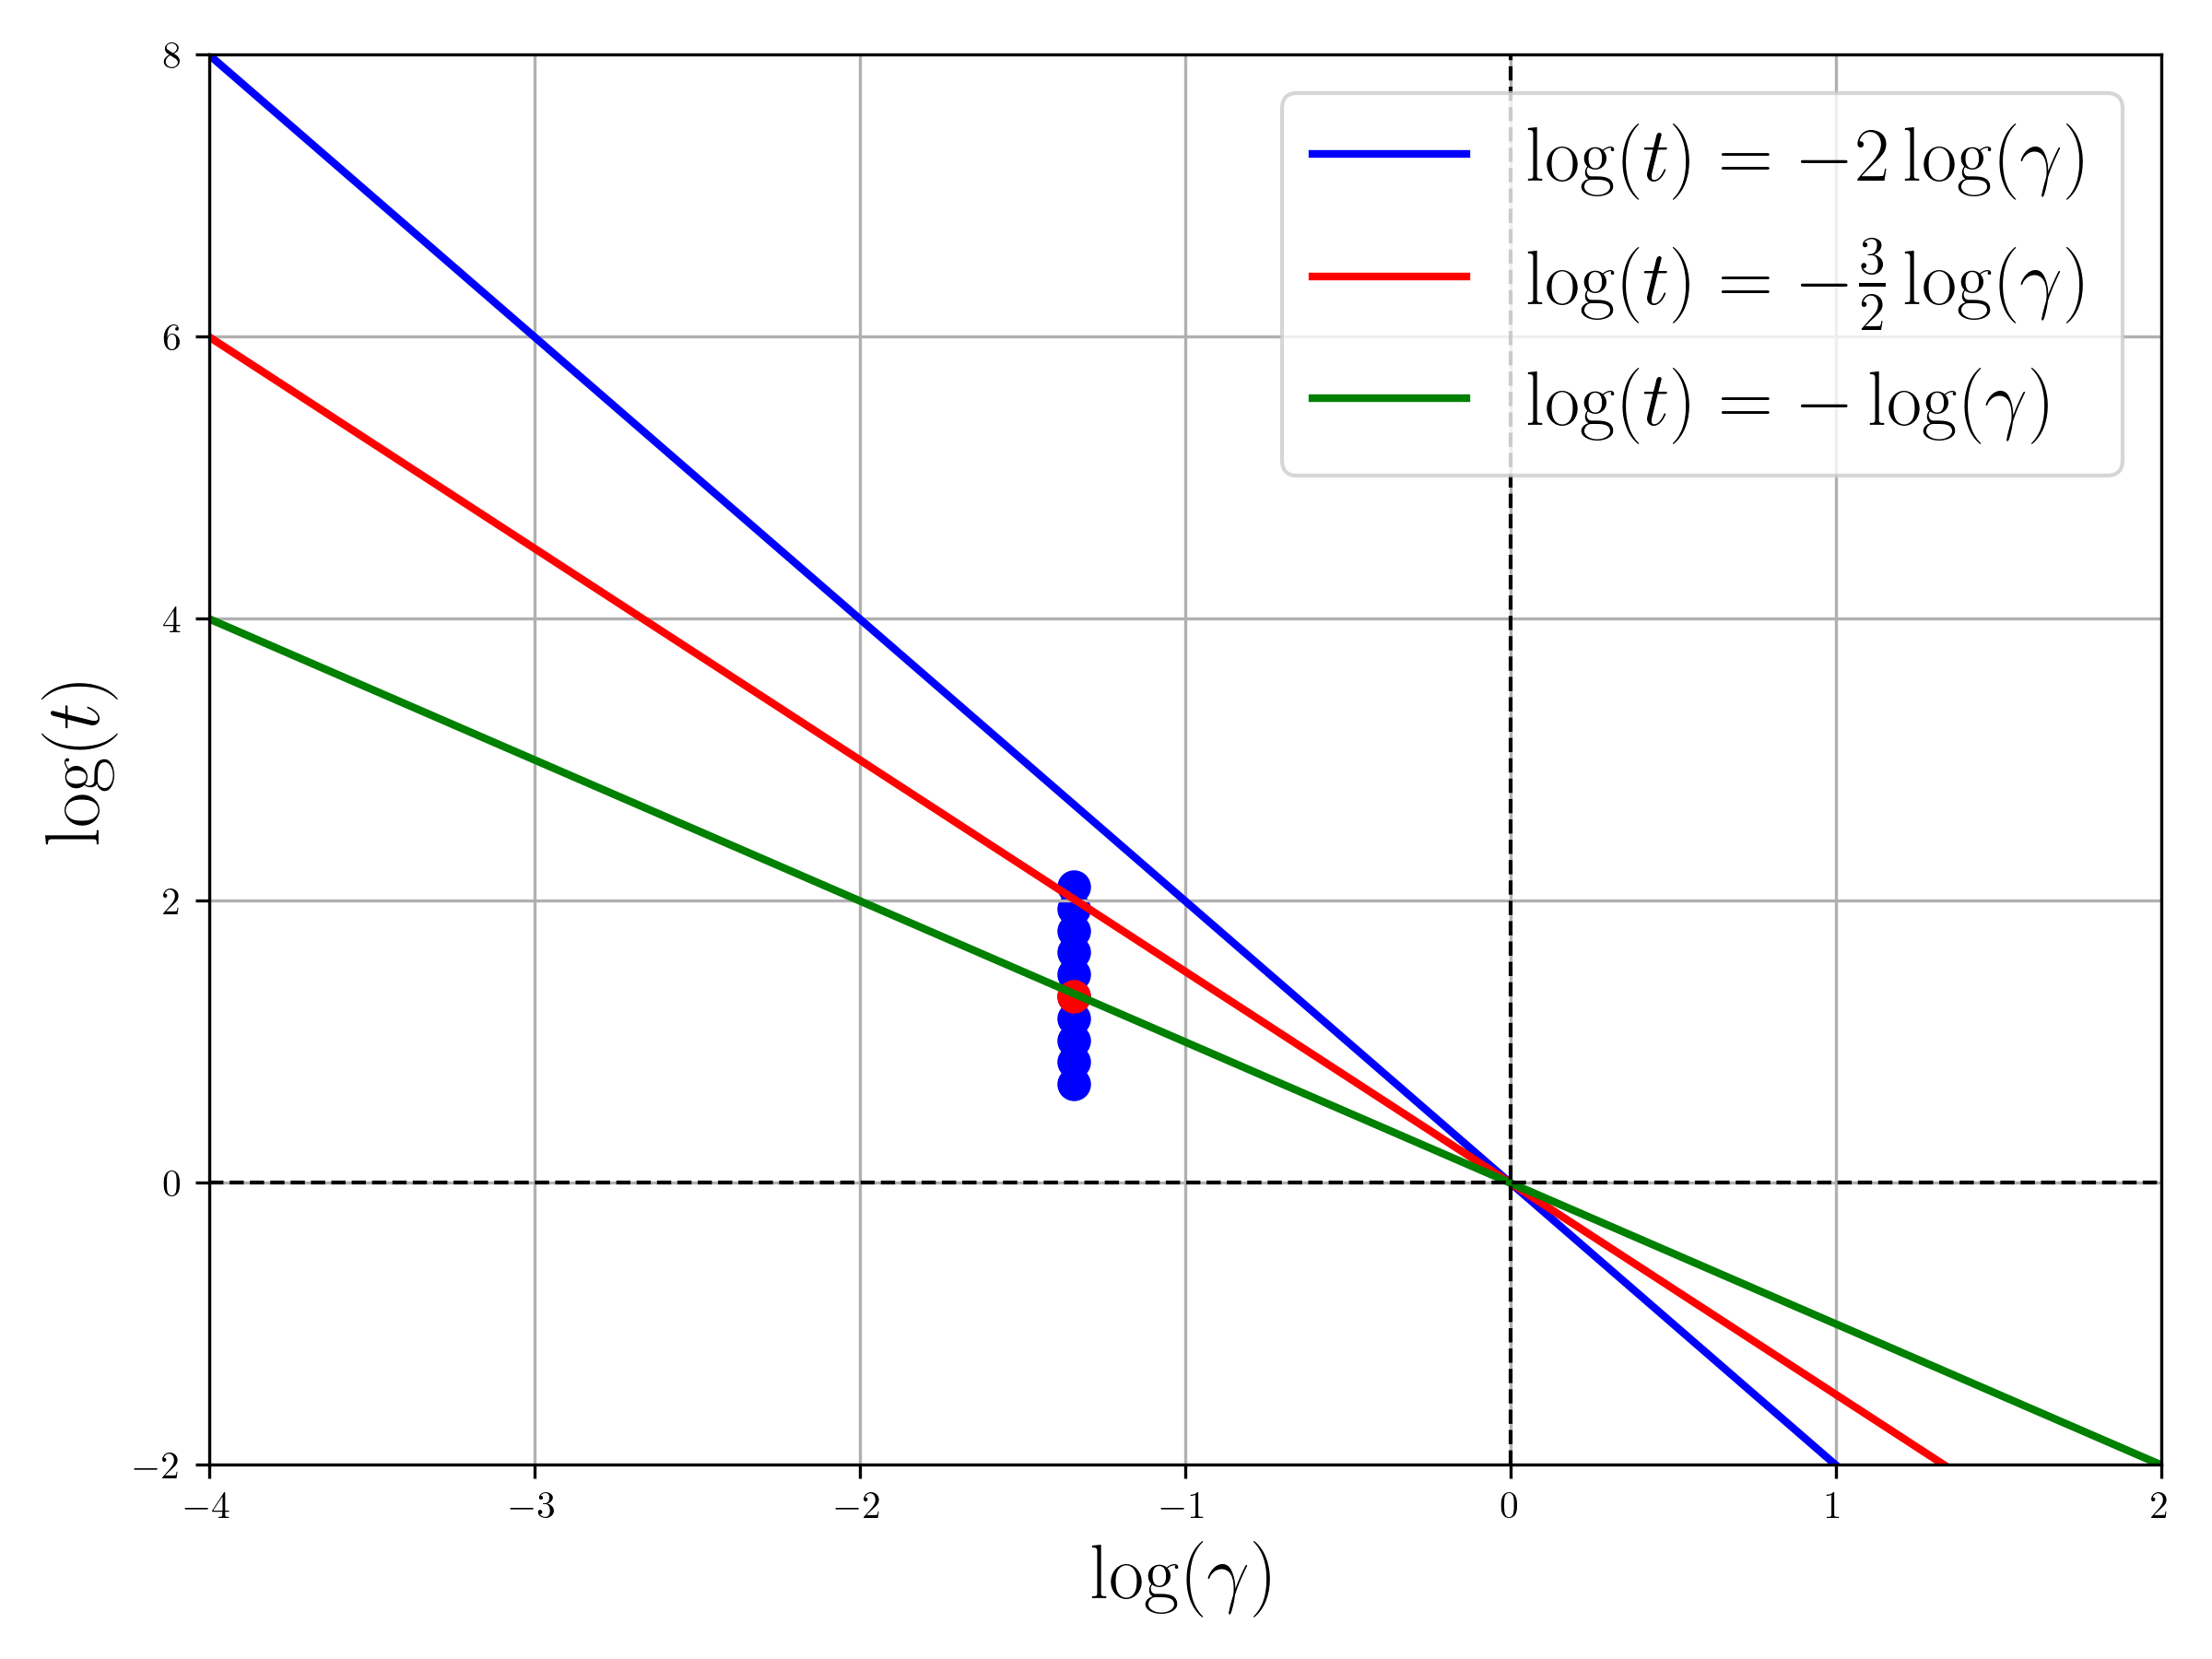
\includegraphics[width=\textwidth]{Figures/diagram.png}
		\caption{}
		\label{fig:diag}
	\end{subfigure}
	\hfill
	\begin{subfigure}[b]{0.45\textwidth}
		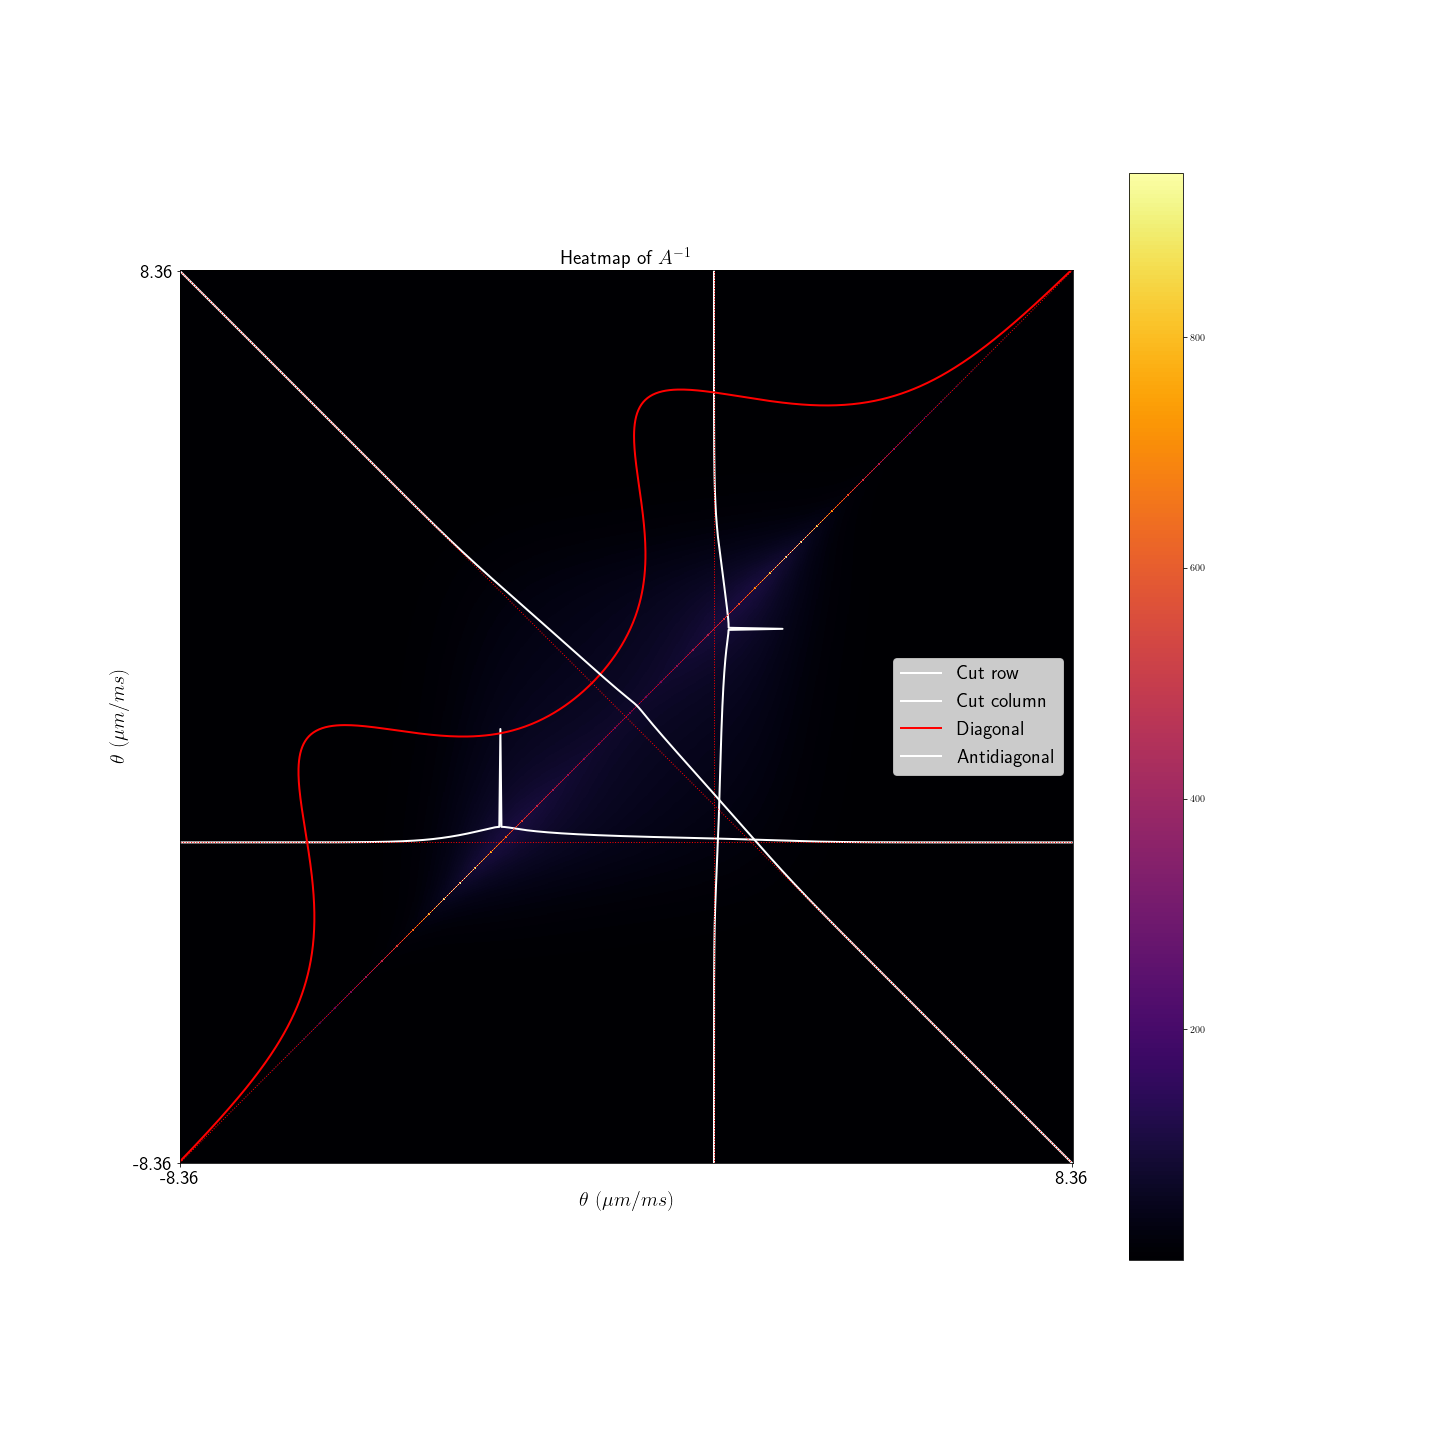
\includegraphics[width=\textwidth]{Figures/fluctu.png}
		\caption{Fluctuations mesurées}
		\label{fig.fluctu.A}
	\end{subfigure}
	\caption{(a) Diagramme de phase du modèle de Lieb-Liniger à l'équilibre thermique. Différents régimes asymptotiques sont séparés par des transitions progressives. %Le passage entre le régime de gaz de Bose idéal et le régime de quasi-condensat a lieu pour \( t \sim \gamma^{-3/2} \), celui entre le régime de quasi-condensat et le régime de bosons impenetrables (hard-core) a lieu pour \( \gamma \sim 1 \), et celui entre le régime hard-core et le gaz de Bose idéal se produit pour \( t \sim 1 \). La ligne en pointillés représente la condition de dégénérescence quantique, qui s’écrit \( t \sim \gamma^{-2} \).% Il est à noter que l'équilibre thermique n’est pas garanti dans le modèle de Lieb-Liniger, en raison de son intégrabilité.
	Le point bleu reprensentent les fluctuation calculer avec $\gamma = m g/\hbar^2 n $ et $t = k_B T/(m g^2/\hbar^2)$. (b) Reprenstation en nuande de couleur des fluctuations $\delta \rho$ avec $T = 60 ~nK$ et $\mu = 27~ nK$ (point rouge dans (b)
}
	\label{fig:diag_fig}
\end{figure}

Et on peux 


\begin{figure}[H]
	\centering 
	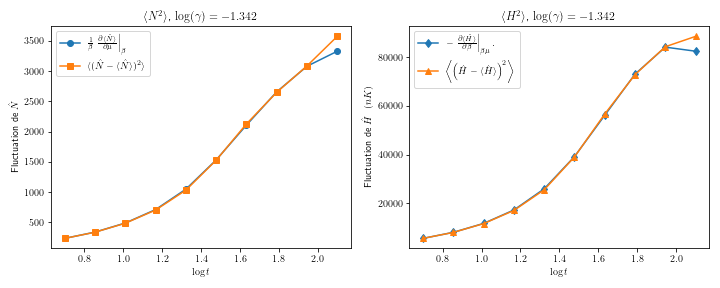
\includegraphics[width=1\textwidth]{Figures/fluctuations_plot_log_gamma=-1.342.png}	
	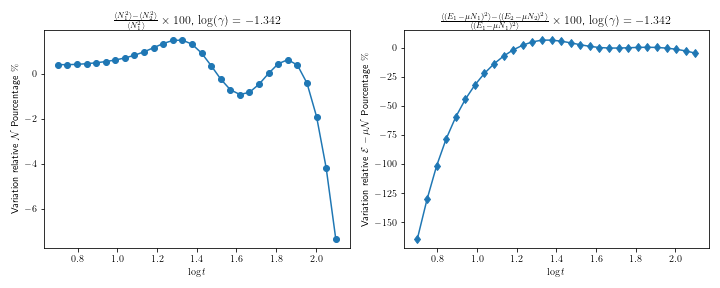
\includegraphics[width=1\textwidth]{Figures/fluctuations_relativ_plot_log_gamma=-1.342.png}	
	\captionsetup{skip=10pt} % Ajoute de l’espace après la légende
	\label{fig.fluctu.A}
\end{figure}



%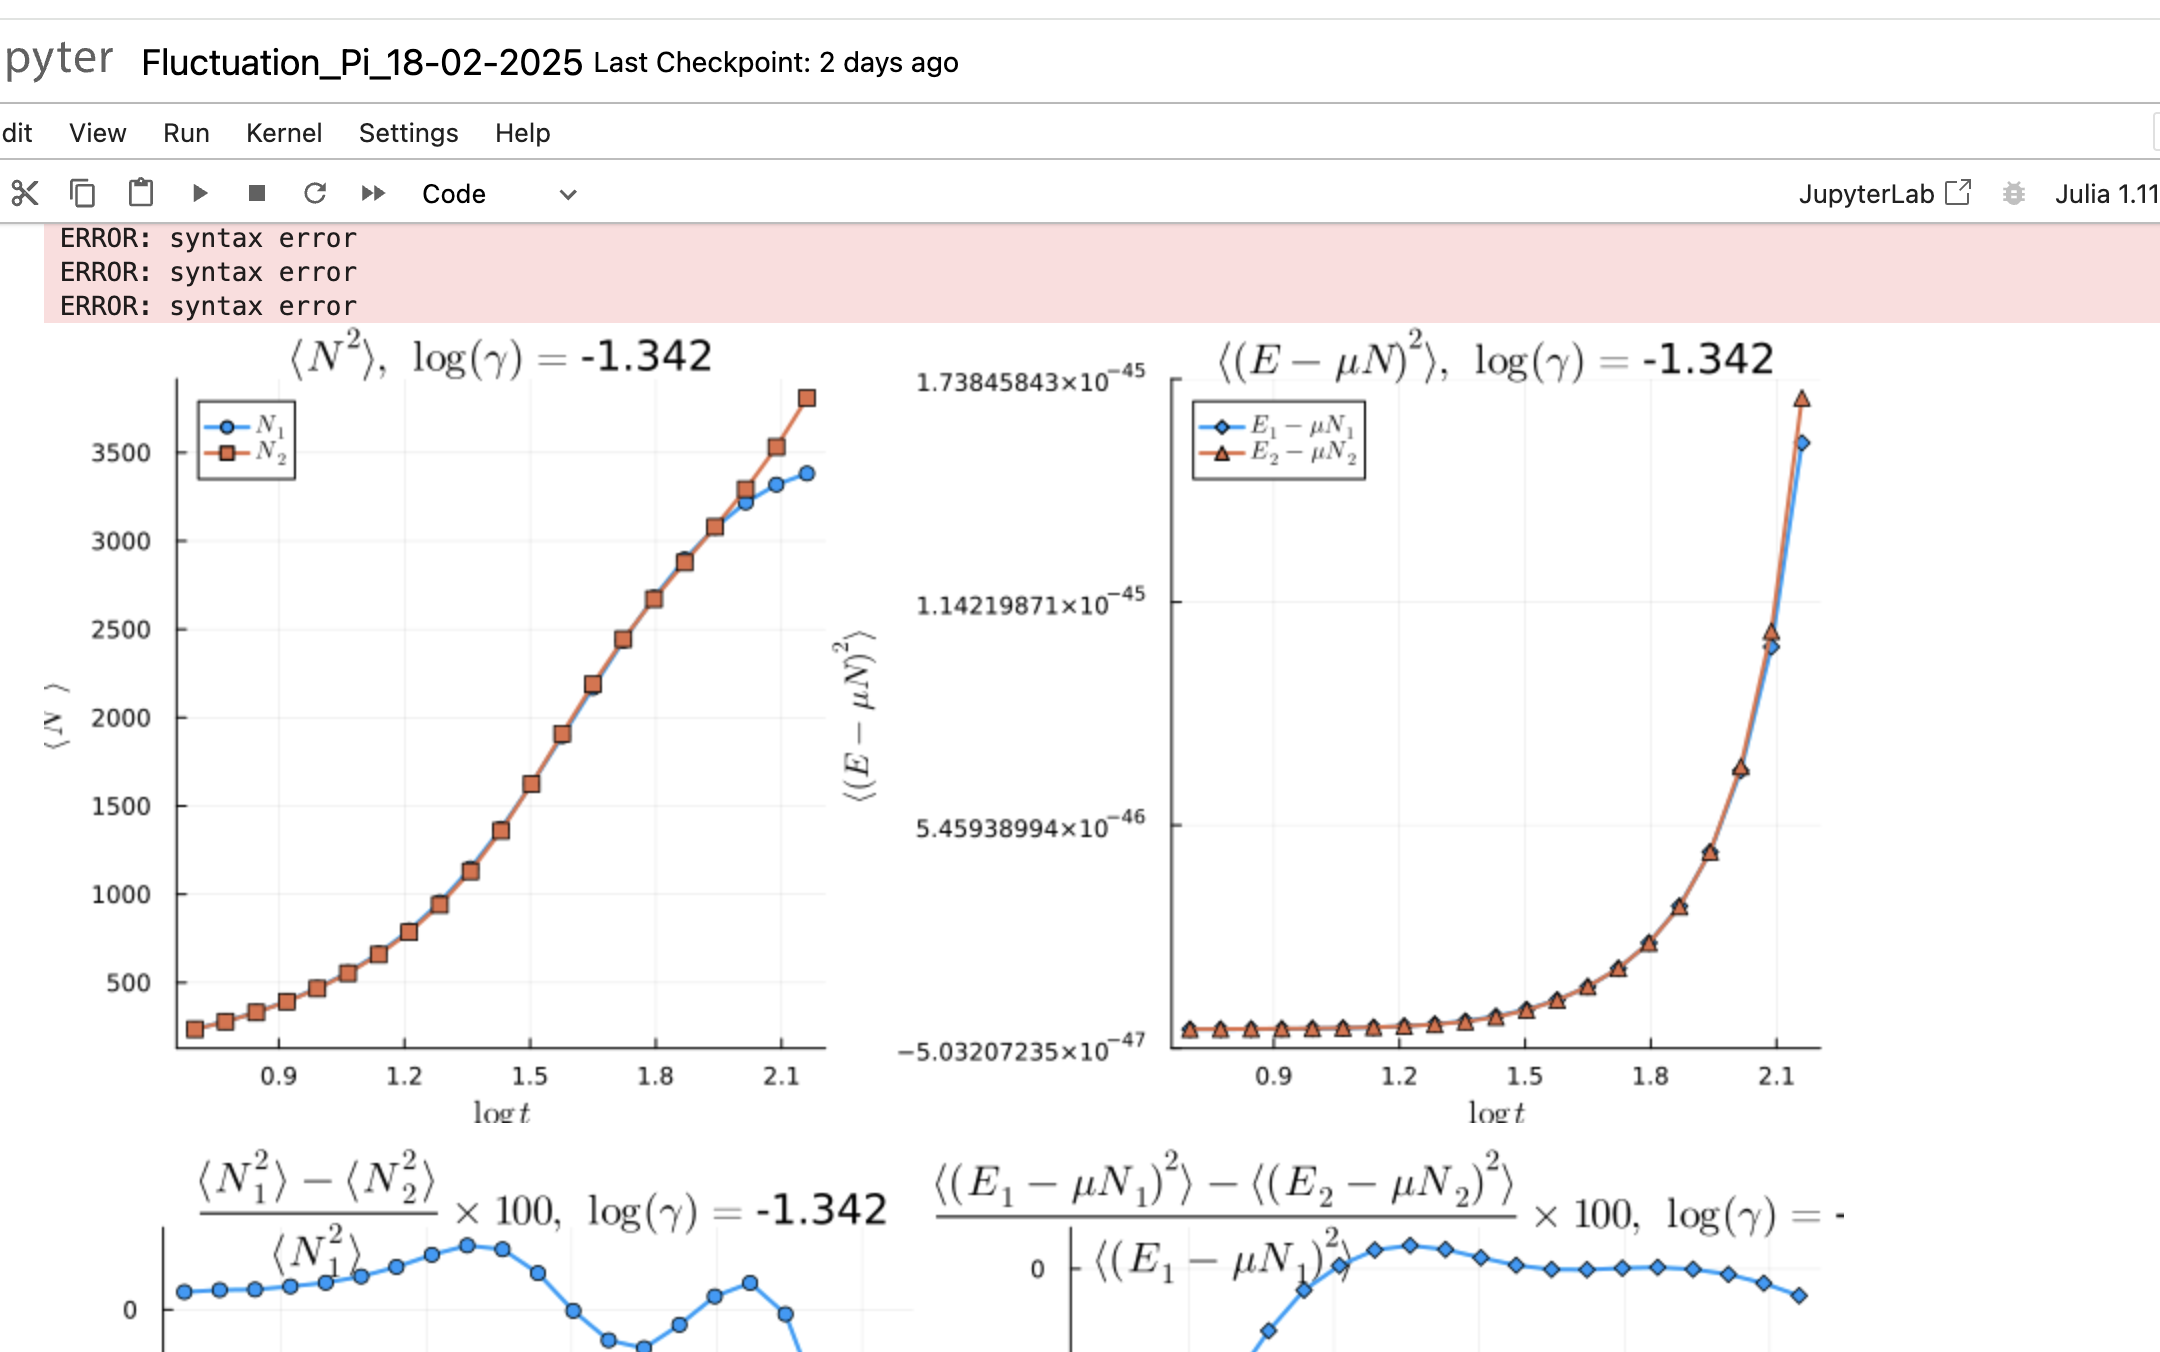
\includegraphics[width=1\textwidth]{Figures/test}

%\begin{aff}
%Donc une a l'ordre un en $\delta \theta (\operator{A}^{(0)})^{-1} %\operator{V}$ 

%\begin{eqnarray*}
%	\langle \delta \Pi ( \theta) \delta \Pi ( \theta') \rangle & = &  ( (\Pi^c_s - \Pi^c)\Pi^c/\Pi^c_s ) ( \theta ) \delta_{\theta, \theta'}/\delta \theta + \mathscr{F}(\theta , \theta' ) ,	
%\end{eqnarray*}

%avec 

%\begin{eqnarray*}
%	\mathscr{F}(\theta , \theta' ) & = & \left [ (\Pi^c_s - \Pi^c )( \theta)  +  (\Pi^c_s - \Pi^c ) ( \theta' )\right ] \frac{\Pi^c}{\Pi^c_s}(\theta)\frac{\Pi^c}{\Pi^c_s}(\theta') \frac{ \Delta( \theta'- \theta )}{ 2 \pi }\\
%	&&  - \left [ (\Pi^c_s - \Pi^c )( \theta)   (\Pi^c_s - \Pi^c ) ( \theta' )\right ] \frac{\Pi^c}{\Pi^c_s}(\theta)\frac{\Pi^c}{\Pi^c_s}(\theta')\int d\theta'' \left (   \frac{ \Pi^c/\Pi^c_s}{\Pi^c_s - \Pi^c} \right )(\theta'') \frac{\Delta(\theta''- \theta)}{2 \pi}\frac{\Delta(\theta''- \theta')}{2 \pi}  	
%\end{eqnarray*}
%\end{aff}



 







